\documentclass{cmc}

\begin{document}

\pagestyle{fancy}
\lhead{\textit{\textbf{Computational Motor Control, Spring 2018} \\
    Python exercise, Lab 2, NOT GRADED}} \rhead{Student \\ Names}

\section*{Student names: \ldots (please update)}

\textit{Instructions: Update this file (or recreate a similar one, e.g.\ in
  Word) to prepare your answers to the questions. Feel free to add text,
  equations and figures as needed. Hand-written notes, e.g.\ for the development
  of equations, can also be included e.g.\ as pictures (from your cell phone or
  from a scanner).  \textbf{This lab is not graded. However, the lab exercises
    are meant as a way to familiarise with dynamical systems and to study them
    using Python to prepare you for the final project.} This file does not need
  to be submitted and is provided for your own benefit. The graded exercises
  will have a similar format.}

\textit{The file \fileref{lab\#.py} is provided to run all exercises in
  Python. Each \fileref{exercise\#.py} can be run to run an exercise
  individually. The list of exercises and their dependencies are shown in
  Figure~\ref{fig:files}. When a file is run, message logs will be printed to
  indicate information such as what is currently being run and and what is left
  to be implemented. All warning messages are only present to guide you in the
  implementation, and can be deleted whenever the corresponding code has been
  implemented correctly.}

\begin{figure}[ht]
  \centering 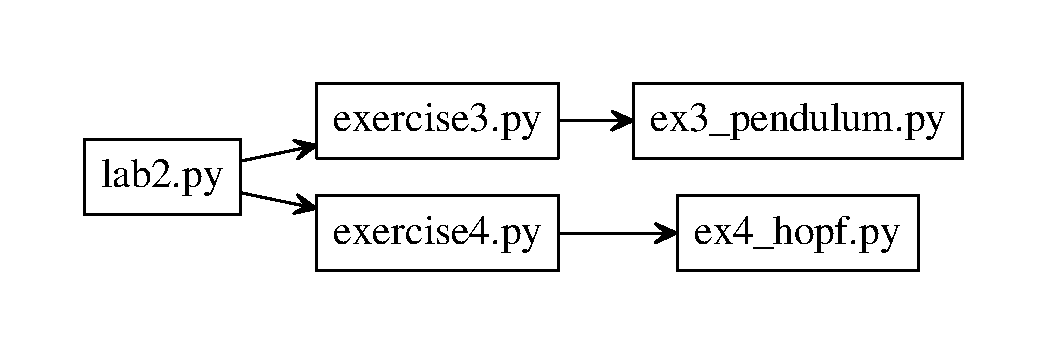
\includegraphics[width=0.5\textwidth]{figures/files}
  \caption{\label{fig:files} Exercise files dependencies. In this lab, you will
    be modifying \fileref{exercise3.py}, \fileref{ex3\_pendulum.py},
    \fileref{exercise4.py} and \fileref{ex4\_hopf.py}.}
\end{figure}

\section*{Question 3: Pendulum with friction}

\subsection*{3.a Find the fixed points of the pendulum with friction
  (i.e. damping), and analyze their stability using a local linearization
  (briefly describe the calculation steps). }


\subsection*{3.b Numerically solve the differential equations of the pendulum
  with different initial conditions.  Show several time evolutions and phase
  portraits with different initial conditions that illustrate several aspects of
  the interesting behavior of the pendulum. See \fileref{exercise3.py} and
  \fileref{pendulum.py} for help with implementation.}


\subsection*{3.c Investigate and describe how the behavior of the pendulum
  changes if friction is zero (d=0).  Show a new phase portrait.}


\subsection*{3.d Does the pendulum without friction (d=0) produce stable limit
  cycles? Discuss, and try to support your statement with some numerical
  simulations (show figures) and/or analytical arguments.}


\subsection*{3.e Investigate how the behavior of the pendulum changes if the
  viscous friction term is replaced with a dry (Coulomb) friction term. Unlike
  viscous friction, dry friction does not depend on speed, only the direction of
  movement. What are the main differences between the two types of pendulum?
  (discuss and show some examples). And is there anything notable about the
  numerical integration of the pendulum with dry friction? If yes, what and why?}

\begin{equation}
  \label{eq:ode-pendulum-dry}
  \dot{\theta} = - {g \over L} \sin \theta - d \cdot sign(\dot{\theta})
\end{equation}


\section*{Question 4: Coupled Hopf oscillators}

\subsection*{4.a Implement a single Hopf oscillator and illustrate its various
  behaviors using time evolution and phase plane figures. See
  \fileref{exercise4.py} and \fileref{hopf.py} for help with implementation.}


\subsection*{4.b Implement a system of two coupled Hopf oscillators and
  illustrate its behavior using figures showing time evolutions of states and of
  angles. You are free to propose your own coupling.  Investigate phase locked
  behavior, and more generally how coupling weights and different parameters
  such as intrinsic frequency affect the global behavior.}


\end{document}